





NEED TO UPDATE THIS SECTION AS PAPER WAS UPDATE ON 2/9 WITH CONTENTS OF USER SESSION MODELING SIMULATION



\chapter{Modeling Landing Page Characteristics for
Mobile Web Access Performance Evaluations on
Object and Page Levels}

\section*{Introduction}
\addcontentsline{toc}{section}{Introduction}
Smart mobile devices with ubiquitous connectivity have become popular worldwide and their utilization has increased the amount of traffic in wireless networks tremendously. 
As mobile users employ their always--present devices to access web--based services, additional forecasts include a shift of the main access of the world wide web from fixed desktops to mobile clients. 
Cisco, Inc. predicts that this current trend will result in a steady growth of mobile data for years to come~\cite{VNI14}.
As the primary means of web access changes, evaluations employing desktop client web access strategies not necessarily reflect the potential for optimizations.
While on the network provider side, caching can readily yield savings through caching~\cite{IhPa11}, the mobile client side becomes increasingly significant due to mobile devices typically exhibiting limitations with respect to battery capacities.
The composition of web pages, e.g., has an impact on battery consumption~\cite{ThAgNiBoSi12}.
Investigating the complexity of web pages, the number of loaded objects were found to positively correlate with the web page load times~\cite{BuMaSe13}, which, in turn will correlate with power consumptions.
Furthermore, in their evaluations the authors found that mobile and non--landing web pages tend to exhibit less complexity. 
In turn, landing pages of popular mobile web sites can be regarded as an upper complexity limit for approximations.

Recent evaluations of web page characteristic developments over time for landing pages of popular fixed and mobile web sites in~\cite{JoSe14Commag} found that mobile versions exhibit around 60 objects and are approaching one Megabyte in size on initial view. 
Images, other media elements (such as Flash or fonts), and Java Script objects were found to be the main overall size contributors.
While energy savings were found to be possible through pre--fetching and caching throughout the mobile age (see, e.g., \cite{SaIs02, ShKuDaWa05,ThChWo13}),
lower cache hit ratios can significantly reduce or inverse potential benefits, see, e.g., \cite{Wang:2012ks,Marquez:2008wf}.
Increasing the difficulty for efficient reduction of wireless network transmissions, a significant portion of web page objects was found to exhibit very short or no cache life time, resulting in additional downloads over the air interface, see, e.g., \cite{JoSe14Commag,Qian:2014dw,JoSe14GreenComm}.
The over--arching problem for higher--level optimization approaches on the mobile client and network sides is to provide a means to model the defining characteristics of web pages requested by mobile device browsers. 
In this contribution, we evaluate the modeling of mobile web pages using a public dataset of popular web pages accessed with a mobile (iPhone) client with respect to their number of objects, sizes, and caching abilities.
We approach this problem for the mobile web by focusing on landing pages as upper limit approximation, following the findings in~\cite{BuMaSe13}. Throughout this chapter, we assume that for caching purposes, only time frames up to a week have the most impact.

\section*{Web Page data sets}
\label{s:data}
\addcontentsline{toc}{section}{Web Page data sets}
We utilize the \url{httparchive.org} data sets of captured web performance metrics, which are publicly available. 
Each of the data sets is generated from initial client views (eliminating caching) of a broad set of popular web sites, which were determined based on the Alexa popularity ranking, accounting for almost 5000 landing pages. 
While the httparchive project gathers and archives the statistics of popular mobile web landing pages, these can be seen as representative upper boundaries of the evaluated characteristics when considered in conjunction with the observations in, e.g.,  \cite{BuMaSe13}.
We utilize the mobile data sets available for Oct. 15, 2013 as our main starting point, but limit the data set to object sizes of at least one byte (e.g., omitting redirects or other types of HTTP messages) and objects exhibiting a cache lifetime of at most one week.

\subsection*{Summary of Data Set Characteristics}
\addcontentsline{toc}{section}{Summary of Data Set Characteristics} 
We provide a high--level overview of the object and web page characteristics of the employed data set in the following.
We denote the number of objects $o$ as $n_o$, the number of web pages as $n_p$, the requests for a specific web page $p$ as $n_{o(p)}$, and the related average as $\overline{n}_{o(p)}$. 

Similarly, we evaluate the individual object size as $x_o$ and their overall average as $\overline{x}_o$.
We denote their aggregated sum on an entire web page as 
\begin{equation}
x_{p}=\sum_{o(p)} x_{o(p)}
\end{equation}
and the average request size for a web page $p$ as  
\begin{equation}
\overline{x}_{o(p)}=\frac{x_{p}}{n_{o(p)}}.
\end{equation}
Furthermore, we evaluate the cache expiration age for individual objects as $t_o$ and denote their average as $\overline{t}_{o(p)}$ when considered in a web page context. 
The fraction of objects with a zero expiration age in cache (i.e., those requiring a download every time) is denoted as $c^0_o$, i.e., 
\begin{equation}
c^0_o=\frac{\sum_o [t_o = 0]}{n_o},
\end{equation}
where $[\cdot]$ denotes the Iverson bracket.
We denote the page level faction as $c^0_{o(p)}$ while independent objects and those within page contexts with potential for caching are denoted as $c_o$ and $c_{o(p)}$, respectively.

We indicate the variability amongst the $n_p=4776$ pages with $n_{o}=197634$ valid object URLs evaluated within the data set employing the Coefficient of Variation (CoV), i.e., the standard deviation relative to the mean. 

We provide the resulting values in Table~\ref{tab:res} for the individual objects and complete mobile web pages.
\begin{table}[]
	\centering
	\caption{Comparisons of the average characteristics $\overline{(\cdot)}$ and the Coefficient of Variation CoV$(\cdot)$ for individual web page objects of the entire data set and the resulting web pages.\label{tab:res}}
	\begin{tabular}{|l||c|c||c|c|}
		\hline
		Metric                    & \multicolumn{2}{|c||}{Objects} & \multicolumn{2}{|c|}{Pages} \\
		& $\overline{(\cdot)}$ &  CoV$(\cdot)$  & $\overline{(\cdot)}$ & CoV$(\cdot)$ \\ \hline
		Objects $o(p)$            &               &        &          60.59          &    0.942     \\ \hline
		
		Sizes $x_o,\overline{x}_{o(p)}$ (kB)        &         12.73        &     2.95     &         12.64         &    1.05     \\ \hline

		Zero cache fraction $c^0_o,c^0_{o(p)}$ &        0.607      &          &        0.649         &  0.455     \\ \hline
		
		Cache fraction $c_o,c_{o(p)}$        &        0.393         &         &        0.351         &  0.844      \\ \hline
	\end{tabular}
\end{table} 
We initially observe that the average number of objects constituting a mobile landing web page is in line with earlier observations made in~\cite{JoSe14Commag}.
We note that the individual object sizes exhibit a fairly high level of variability around their average of 12.73 kB.
After aggregating objects contextually to evaluated web pages, we note that while the average size per page remains close, the variability on the page level is cut by approximately two thirds.

When comparing the potential for caching of the web page objects based on their defined expiration age, we derive from Table~\ref{tab:res} that over 60 \% of items individually and about 65 \% on average on a web page cannot be cached by default. 
A low CoV indicates that on a page level, little difference exists between pages with respect to their average object cache life times. 
The main differences in these characteristics when compared to those described in~\cite{JoSe14Commag} stem from the modified assumptions for the underlying data set, which here includes all mobile pages, but limits the objects based on their expiration ages.
In the following, we evaluate the interplay of these object characteristics in greater details.

\subsection{Evaluation of Object-- and Page level Dependencies}
\addcontentsline{toc}{subsection}{Evaluation of Object-- and Page level Dependencies}
We evaluate the dependencies of cache lifetimes, object sizes, as well as their aggregation into pages in Figure~\ref{fig:rel}.
We note that throughout the remainder of this paper, we illustrate the results using an aggregation level of 1000 bytes for object sizes and 900 seconds for object expiration ages for visual clarity only (i.e., not impacting underlying calculations).

\begin{figure*}[b!]
	\centering
	\subfloat[Individual mobile web page objects	\label{fig:orel}]{\includegraphics[width=2.75in]{scatterplots/overall_2d_scatterplot_respSizes_expAges-eps-converted-to}}
	\hfil
	%\qquad
	%
	\subfloat[Mobile Web Pages \label{fig:prel}]{\includegraphics[width=2.75in]{scatterplots/scatter}}
	%
	\caption{Individual sizes and cache expirations for 197634 web objects as well as their averages when considering page--level relationships for 4776 mobile web landing pages.\label{fig:rel}}
\end{figure*}

Initially, we observe that the distribution of object sizes over their lifetime is spread across the entire range of evaluated times. 
We secondly note that at specific expiration times, i.e., none, hour, day, etc., a broader range and aggregation of objects can be observed. 
While we do not observe a close correlation of object sizes and their cache lifetimes, we note that large numbers of even large sized objects have a very short lifetime.

Next, we evaluate the aggregated sizes on a page level in Figure~\ref{fig:prel}, whereby we focus on the range of below 100 objects, expiration below the first several days of a week, and up to 100 kB object sizes.
We observe that the majority of web pages in this group exhibits a low average expiration age as well as a generally small average object size.
We additionally observe that the number of objects on a web page is fluctuating widely for this data set.
Overall, we do not observe a direct relationship between the number of objects, their overall sizes, and their expiration ages once we evaluate them contextually combined on the web page level.
We employ this observation in the following modeling approach.


\section{Object--Level Modeling}
\addcontentsline{toc}{section}{Object--Level Modeling}
\label{s:object}
The initial modeling approach targets the level of individual objects as present in the entire data set, i.e., across all mobile web pages. 
This approach hence would be suitable for high--level modeling of mobile web traffic characteristics.

\subsection{Object Sizes}
\addcontentsline{toc}{subsection}{Object Sizes}
The individual object sizes follow a Weibull minimum distribution, which we employ to randomly draw individual object sizes $x_o$ as defined by 
\begin{equation}\label{eq:weibull}
f\left(x_o\right) = \frac{a}{\lambda} \left(\frac{x_o}{\lambda}\right)^{a-1} \cdot e^{-(x_o/\lambda)^a}, 
\end{equation}
with $x_o>0, \alpha>0$.
We identified the shape parameter as $a \cong  0.573$ and the scale parameter as $\lambda \cong 8887.5$.
We illustrate the results from 500 evaluations in Figure~\ref{fig:osize}, noting that we omit the illustration of the confidence intervals for readability (they are typically within ten percent of the original value).

We observe that both distributions peak at a small response size on drop immediately, with the simulated web page object sizes following the trend of the underlying data set closely.
Due to the nature of the selected Weibull distribution for simulation purposes, the smaller abrupt changes in the distribution of sizes visible for the source data, e.g. between object sizes of 10 kB and 20 kB, are not captured in the modeled distribution.
We reason that the tractability and otherwise close fit, however, outweigh the capturing of these minor irregularities.


\subsection{Object Expiration Ages}
\addcontentsline{toc}{subsection}{Object Expiration Ages}
Next, we evaluate the capturing of the expiration ages, i.e., the maximum cache lifetime, of the individual web objects found in the dataset.
The underlying notion of web server configurations exhibits a non--linear relationship between the individual object expiration times set $t_o$, whereby common time frames, such as mandatory hourly or daily refreshes of individual objects are common. 
In turn, the modeling of this particular behavior follows a piecewise approximation, which distributes the expiration ages based on their original frequency in the underlying data set within the one week time interval we consider here.
Denoting $U(a,b)$ as a continuous uniform distribution between inclusive $a$ and $b$ and $U[a,b]$ its discrete counterpart, we model the mobile web object expiration times by initially drawing $\tau_o \sim U(0,1)$ randomly.
We subsequently determine the expiration age $t_o$ for the object under consideration as in Eq.~\ref{eq:t0}.
\begin{equation*}\label{eq:t0}
t_o =
\begin{cases}
0 ~\mathrm{for}~ 0 \le \tau_o <  0.6108,\\
300 ~\mathrm{for}~ 0.6108 \le  \tau_o < 0.6235,\\
600 ~\mathrm{for}~ 0.6235 \le \tau_o < 0.6353,\\
900 ~\mathrm{for}~ 0.6353 \le \tau_o < 0.6460,\\
3600 ~\mathrm{for}~0.6460 \le \tau_o < 0.6887,\\
7200 ~\mathrm{for}~0.6887 \le \tau_o < 0.6970,\\
14400 ~\mathrm{for}~0.6970 \le \tau_o < 0.7070,\\
21600 ~\mathrm{for}~0.7070 \le \tau_o < 0.7152,\\
43200 ~\mathrm{for}~0.7152 \le \tau_o < 0.7333,\\
86400 ~\mathrm{for}~0.7333 \le \tau_o < 0.8037,\\
172800 ~\mathrm{for}~0.8037 \le \tau_o < 0.8126,\\
604800 ~\mathrm{for}~0.8126 \le \tau_o < 0.8909,\\
U[0, 604800]~\mathrm{otherwise}.
\end{cases}
\end{equation*}

\begin{figure}[b!]
	\centering
	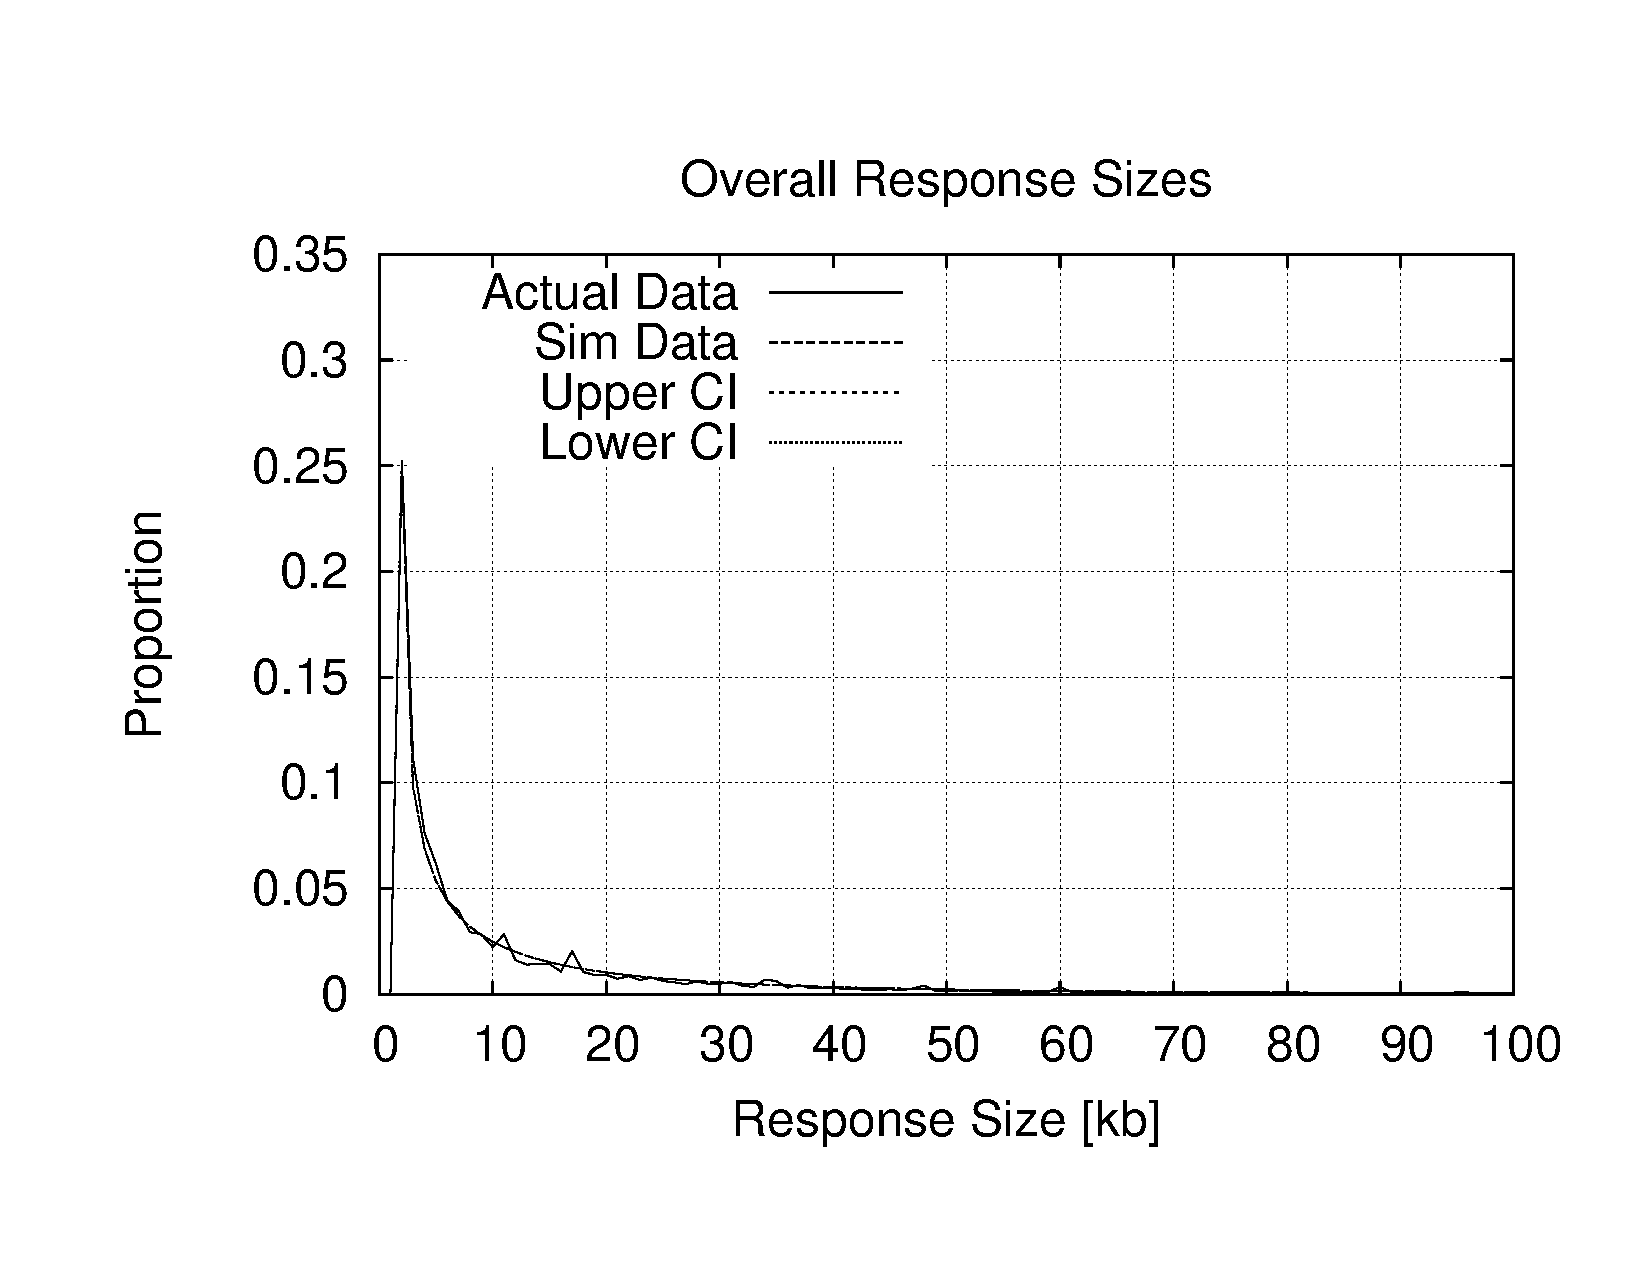
\includegraphics[width=.33\textwidth,angle=270]{respSizes/Overall/overall_respSizes}
	\caption{Real data set and synthetically generated web page object sizes across the entire data set.}
	\label{fig:osize}
\end{figure}

We illustrate the original data set and simulated values in Figure~\ref{fig:oexp}.
\begin{figure}[b]
	\centering
	\includegraphics[width=.33\textwidth,angle=270]{expAges/Overall/overall_expAges-eps-converted-to}
	\caption{Real data set and synthetically generated web page object expiration ages across the entire data set.}
	\label{fig:oexp}
\end{figure}
We observe that the original expiration times exhibit several ``spikes'' of higher probability at the common time instances for mandatory cached element refreshes. 
This trend of expirations motivates a piece--wise approximation instead of fully capturing the detailed characteristics for the entire time scale.
Our model approaches the generally compartmentalized structure of expiration times especially for the shorter time scales of common values and coarsely approximates the longer tail end with smaller numbers of objects.


\section{Page--Level Modeling}
\addcontentsline{toc}{section}{Page--Level Modeling}
\label{s:page}
The modeling of the web pages is based on the combination of modeling the number of objects, their sizes, and their expiration times.
In contrast to the individual object level, we now need to consider the mobile web page--level context for the expiration age distributions, especially those objects that cannot be cached.
In the following, we present the individual model approach by the respective component.

\begin{figure}[t!]
	\centering
	\subfloat[Average number of objects per mobile web page	\label{fig:preq}]
	{\includegraphics[width=.34\textwidth,angle=270]{numResponses/numResponses-eps-converted-to}}
	\qquad
	\vspace{.1in}
	%
	\subfloat[Mobile web page sizes\label{fig:psize}]
	{\includegraphics[width=.34\textwidth,angle=270]{respSizes/PageLevelTotal/page_level_sum_respSizes-eps-converted-to}}
	\qquad
	\vspace{.1in}
	%
	\subfloat[Average mobile web page object expiration\label{fig:pexp}]
	{\includegraphics[width=.34\textwidth,angle=270]{expAges/PageLevelAverages/PageLevelexpAgeAverage/page_level_average_expAges-eps-converted-to}}
	\qquad	
	\vspace{.1in}
	%
	\caption{Page--level simulation of mobile web landing pages for the October 15, 2013 data set.\label{fig:pages}}
\end{figure}

\subsection{Number of Objects per Page}
\addcontentsline{toc}{subsection}{Number of Objects per Page}
The evaluation of the aggregated object numbers $n_{o(p)}$ for the individual pages $p$ indicates a distribution that follows a general Gamma distribution as 
\begin{equation}\label{eq:gg}
f\left( n_{o(p)} \right) = \frac{ k \cdot (n_{o(p)})-\gamma)^{\kappa\alpha-1} }{\beta^{\kappa\alpha}\Gamma(\alpha)}e^{-\left(\frac{n_{o(p)}-\gamma}{\beta}\right)^\kappa},
\end{equation}
whereby we determine the two shape parameters as $\alpha=3.1119, \kappa=0.6167$, the scale parameter $\beta=8.2912$, and the location parameter as $\gamma=0.17238$.
​
We illustrate the resulting outcome in Figure~\ref{fig:preq} as a comparison between original and simulated data, as well as the  width of the confidence interval in relation to the simulated data.
We observe that the average number of objects per page in both the original and simulated page data sets exhibit the same sharply rising distribution with a significantly longer tail of pages comprised of more than 25 objects.
We furthermore observe that the relative confidence interval width exhibits an increasing trend as the number of objects increases up to about 8 \%. 
This trend originates in the increasingly smaller probabilities of attaining a high number of web page elements. In turn, small deviations have an increasing impact on this relative performance metric. 



\subsection{Average Mobile Web Page Size}
\addcontentsline{toc}{subsection}{Average Mobile Web Page Size}
With the determined number of objects in a page, the next step considers the determination of the individual web page object sizes.
The individual object size on the page level is determined in a next step by employing a Weibull distribution (as in Equation~\ref{eq:weibull}) with $a=0.27 ,\lambda=700$, and location adjusted by 2.5.
The resulting sum of mobile web landing page objects sizes is illustrated in Figure~\ref{fig:psize}.
We observe that the page size distribution for both original and simulated data  exhibits the same trend of mostly smaller web page sizes paired with a long tail end.
The most notable difference between the two data sets occurs in the range of smaller web page sizes below 500 kB, where the original data has a less pronounced peak than the simulated data.
The relative confidence interval values follow the same trend we previously observed in Figure~\ref{fig:preq} for the number of requests.
Specifically, the relative width of the confidence interval increases with the page sizes and the decline of their respective probability.
We follow the prior reasoning that the significantly reduced probability towards the tail end is responsible for this increasing trend.  


\subsection{Average Mobile Web Page Expirations}
\addcontentsline{toc}{subsubsection}{Average Mobile Web Page Expirations}
As a last step, we determine the expiration ages for the individual web page objects, but now with a contextual consideration for their distribution within the underlying mobile web pages as $t_o^p$.
We separate pages into different categories as ($i$) current, ($ii$) short--lived, ($iii$) medium--lived, and ($iv$) regular.

\subsubsection{Current Pages}
\addcontentsline{toc}{subsubsection}{Current Pages}
Current pages are characterized by all of their objects exhibiting a zero cache lifetime, and thus require extensive downloads. 
They account for approximately 6.3 \% of the pages in the simulated data set.

\subsubsection{Short--lived Pages}
\addcontentsline{toc}{subsubsection}{Short--lived Pages}
This page category exhibits a low expiration age for all its objects and accounts for approximately 24.1 \% of all pages.
The expiration age for all objects is determined following the piece--wise approach in Equation~\ref{eq:t0}, but with modified ranges and probabilities as in Equation~\ref{eq:t1} as 
\begin{equation}\label{eq:t1}
t_{o(p)} =
\begin{cases}
300 ~\mathrm{for}~ 0 \le \tau_o < 0.088, \\
1200 ~\mathrm{for}~ 0.088 \le \tau_o < 0.158, \\
1800 ~\mathrm{for}~0.158\le \tau_o < 0.246,\\
3600 ~\mathrm{for}~0.246 \le \tau_o < 0.351,\\
7200 ~\mathrm{for}~0.351 \le \tau_o < 0.404,\\
14400 ~\mathrm{for}~0.404 \le \tau_o < 0.456,\\
21600 ~\mathrm{for}~0.456 \le \tau_o < 0.474,\\
U[0, 604800]~\mathrm{otherwise}.
\end{cases}
\end{equation}

\subsubsection{Medium-lived Pages}
\addcontentsline{toc}{subsubsection}{Medium-lived Pages}
The long--lived page category exhibits a heavier tail for the expiration ages of its objects.
In turn, we employ a log--logistic distribution to model the expiration ages of all objects as 
\begin{equation}
f(t_{o(p)})=\frac{\beta}{\alpha} \left(\frac{t_{o(p)}-\gamma}{\alpha}\right)^{\beta-1}\left(1+\left(\frac{t_{o(p)}-\gamma}{\alpha}\right)^\beta\right)^{-2},
\end{equation}
whereby we set scale parameter $\alpha \approx 0.889 $, shape parameter $\beta \approx 2600.7$, and location parameter $\gamma=1$. 
When drawing a random expiration age, we limit the upper end of expiration ages to 43200.

\subsubsection{Regular Pages}
\addcontentsline{toc}{subsubsection}{Regular Pages}
Regular pages account for the majority 63.3 \% of the simulated web pages. 
Their simulation is a two--step process, which initially determines the number of non--cacheable objects $c^0_{o(p)} \in [0,1]$ as a sample from a normal distribution with $\lambda \approx 0.629, \sigma \approx 0.301$.
In a second step, the remaining expiration ages are set according to 
\begin{equation*}
t_{o(p)} =
\begin{cases}
	0	~\mathrm{for}~	0.000	\le \tau_o <	0.611,                \\
	43200	~\mathrm{for}~	0.611	\le \tau_o <	0.629,            \\
	U[43201,86400]	~\mathrm{for}~	0.629	\le \tau_o <	0.641,   \\
	86400	~\mathrm{for}~	0.641	\le \tau_o <	0.885,            \\
	U[86401,172800]	~\mathrm{for}~	0.885	\le \tau_o <	0.889,  \\
	172800	~\mathrm{for}~	0.889	\le \tau_o <	0.898,           \\
	U[172801,259200]	~\mathrm{for}~	0.898	\le\tau_o <	0.900, \\
	259200	~\mathrm{for}~	0.900	\le \tau_o <	0.908,          \\
	U[259201,604800]	~\mathrm{for}~	0.908	\le \tau_o <	0.922, \\
	604800	~\mathrm{otherwise}.
\end{cases}
\end{equation*}

Comparing the thus generated expiration times with those found in the original data set in Figure~\ref{fig:pexp}, we observe that the average page object expiration ages follow the same decreasing trend.
We furthermore note that the underlying data set exhibits a significantly higher level of variability in the average page object expiration ages than the simulated data. 
Additionally, we also observe that the simulated data features a slightly increased probability of shorter average expiration ages up to a day.
We note that the relative confidence interval width increases from very narrow to a steady 20 \% of the simulated data 
for the tail end of the average page level expiration ages. 
As visible, here the underlying dataset itself exhibits significant variability, which together with the lower probabilities can be regarded as the main source for the heightened relative confidence interval width.

\section{Evaluation}
\addcontentsline{toc}{section}{Evaluation}
\label{s:eval}
We now employ our model to evaluate its capability to capture web caching characteristics as outlined in, e.g., \cite{JoSe14GreenComm}, through simulations.
We initially assume that all web page objects in the data set have to be cached and evaluate the amount of resulting data that remains in the cache, employing our model in 1000 simulations. 
We compare the results to the original dataset in Figure~\ref{fig:simoct13}.  

(We additionally note that we omit confidence intervals for clarity, as their width is typically within 1 \%).
We observe that the original cached data amount quickly reduces to only about 45 \%, which is attributed to the frequent immediate expiration of objects.
As time progresses, the amounts of data that remain in the cache exhibit a staircase behavior, increasing at common time boundaries, such as an hour or a day.
We note that the simulated cached contents are initially underestimated, by a margin of about 10 \%. 
As time progresses, the model--based estimation follows the original data's trend and slightly underestimates the cached data amounts approximately after 30 minutes.
We observe that the underestimation, however, remains close to the original data, with deviation peaking around 5 \%.

\begin{figure}
	\centering
	\includegraphics[width=.33\textwidth,angle=270]{modeling_months_cache/oct13/mobile_bytes_graphs-eps-converted-to}
	\caption{Results from evaluations 1000 cache simulations employing the model for Oct. 15, 2013. Our model captures the trends for the overall amounts in the cache over time.\label{fig:simoct13}}
\end{figure}

Overall, we conclude that our model successfully captures the overall trend for the objects of mobile landing web pages, including the approximation of cached amounts data over time. 

\section{Conclusion}
\addcontentsline{toc}{section}{Conclusion}
\label{s:conc}
We described an approximation to model the behavior of popular mobile web landing pages, which are used as upper limit approximation of data that can be expected to require networked delivery to mobile clients.
Our model is based on the assumption that the distribution of object expirations over time does not change significantly as time progresses, but the composition of web pages rather is sensitive to size changes.

We employ this approach to derive a time--independent approach to the application of our model, which is able to predict the cached amounts or downloaded amounts that are required when considering a large number of popular web pages.
As our model slightly under--estimates the amount of data remaining in a potential cache for up to 30 minutes, its resulting output can be readily applied in that time frame, whereas larger time frame model outputs slightly overestimate the cached amount and require discounting.
In future works, we intend to evaluate the model on a finer--grained approach, incorporating the different types of objects constituting the simulated mobile pages.